\chapter{Theory}
The required background theory will be presented in a top-down approach. For someone experienced in the field of sEMG and signal processing some portions can be perceived as ubiquitous but it is done to make this paper more accessible for readers from different fields.

\section{Force estimation from sEMG}
When moving a limb the most intuitive way of describing it is a change in position, moving your hand from A to B. However, a more objective way of describing this movement is in terms of forces applied on a mass \cite{human_physiology,human_anatomy_physiology,3d_printing_soft_semg}:
\begin{itemize}
    \item The brain makes decision to move a limb and sends a signal through motor neurons
    \item The synaptic input received from the motor neuron results in contraction of the muscles
    \item This (simply put) causes a force to be applied on a mass, or a torque around a pivot point
    \item This force results in an acceleration in a certain direction
    \item This acceleration is maintained for a certain period of time
    \item The entire process is repeated for deceleration using visual, kinesthetic, proprioceptive and tactile sensory signals \cite{human_robotics}
    \item Your limb has arrived at a new location.
\end{itemize} 

Understanding this reasoning of moving a limb in terms of forces being applied by contracting muscles is vital because it forms the basis for recognizing a user's intent. EMG can be used to measure the intensity of muscle activation which indicates the amount of contraction \cite{human_robotics}. By measuring the amount of contraction of two antagonistic muscles it is possible to calculate the amount of force applied in a certain direction. Even if the limb is replaced by a prosthesis this idea of forces moving a mass will still apply, and thus EMG can be used as a human-machine interface.

So to summarize the basic concept of force estimation:
\begin{itemize}
    \item Movement of a limb is the result of a net force acting on that limb
    \item This net force is the result of certain muscles contracting stronger than other muscles
    \item The contraction of these muscles follows from muscle activation 
    \item Muscle activation can be measured using EMG
    \item EMG can be used to estimate limb movement
\end{itemize}

\begin{figure}[h!t]
	\begin{center}
		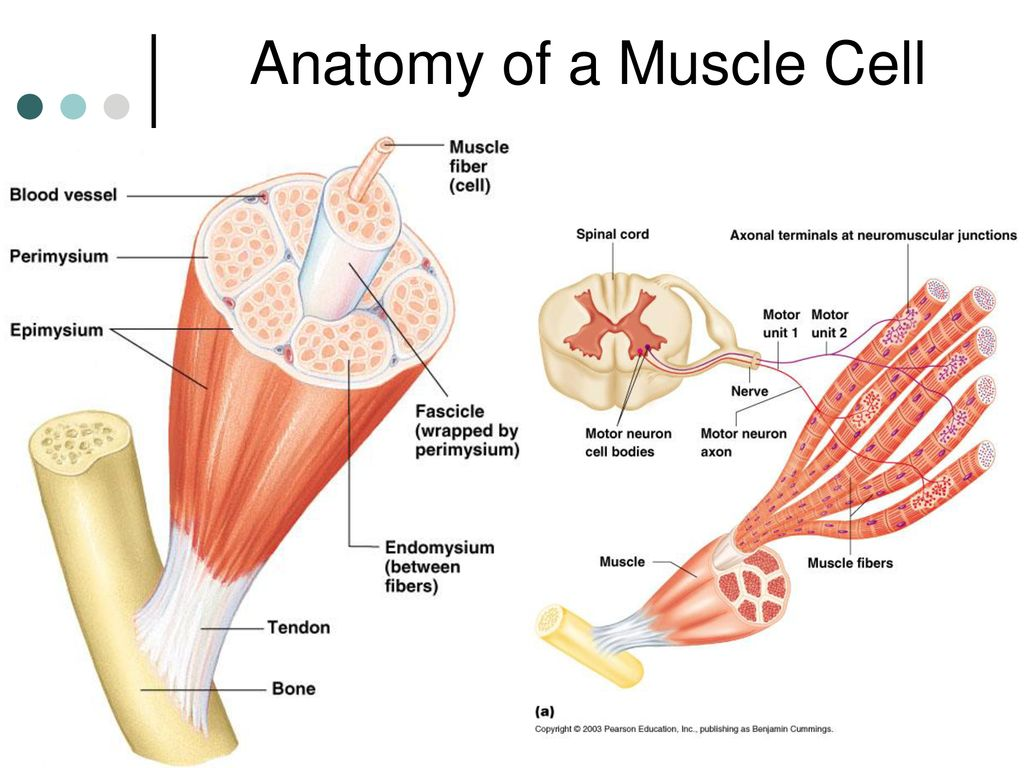
\includegraphics[width=0.7\columnwidth]{images/anatomy_of_a_muscle_cell.jpg}
	\end{center}
	\caption{Anatomy of a muscle \cite{human_anatomy_physiology}.}
	\label{fig:muscle_anatomy}
\end{figure}


Figure~\ref{fig:muscle_anatomy} illustrates the anatomy of a muscle. 
Large skeletal muscles such as the biceps consists of hundreds of thousands of small muscle fibers. These muscle fibers are divided into groups called motor units, and each motor unit is connected to a motor neuron which is a special type of very long brain cell that runs through the spinal cord. A contraction of a skeletal muscle is the result of many muscle fibers contracting individually and repeatedly \cite{human_anatomy_physiology}. The contraction of these muscle fibers is the result of muscle activation which in turn is the result of an action potential caused by the motor neuron. The activation of the muscle fibre is a small yet measurable voltage. When measuring the surface EMG of an activating skeletal muscle the result is the aggregate of the small voltages from all activating muscle fibers. This manifests itself into a signal resembling white noise where the amplitude of the noise correlates to the number of activated muscle fibers and thus to the amount of contraction the skeletal muscle will experiences \cite{optimal_myoprocessor}. An illustration of the form of the measured sEMG is shown in Figure~\ref{fig:sEMG_signal_example} where a maximum voluntary contraction (MVC) is measured from a biceps.
 
\section{sEMG signal properties}
\begin{figure}[h!t]
	\begin{center}
		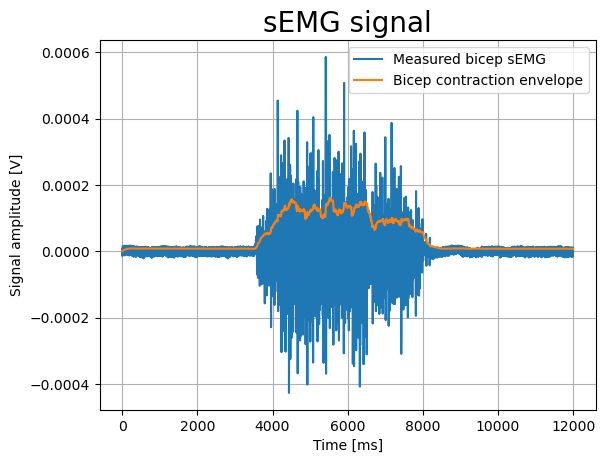
\includegraphics[width=0.7\columnwidth]{images/sEMG_signal_example.png}
	\end{center}
	\caption{sEMG signal measured from bicep during contraction}
	\label{fig:sEMG_signal_example}
\end{figure}

To summarize: to determine the degree of activation of a skeletal muscle we simply need to determine the amplitude of the noise at the surface of the muscle.

From this point onward 'noise' will refer to the generated by muscle contraction as 'the signal'. the reason for this is that noise is usually unwanted, but the signal caused by muscle contraction is the opposite of unwanted: It precisely what sEMG is trying to measure! 

Unfortunately, when measuring sEMG signals it is impossible to measure solely the signal generated by muscle contraction. The signal may be contaminated by other signals coming from the surrounding environment (such as \SI{50}{\Hertz} power lines nearby) or from the amplifier used to amplify the measured signal. So in reality we are measuring a combination of our desired signal from muscle contraction, and the undesired noise from the environment and amplifier. An illustration of the frequency content of the signal and noise is shown in Figure~\ref{fig:sEMG_fft_signalnoise_example}. Note how the noise has large peaks at \SI{50}{\Hertz} and multiples of \SI{50}{\Hertz}; This is the noise generated by the power lines. 

\begin{figure}[h!t]
	\begin{center}
		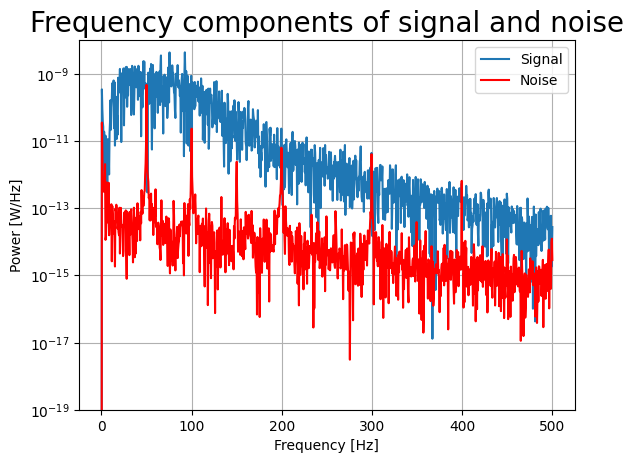
\includegraphics[width=0.7\columnwidth]{images/sEMG_fft_signalnoise_example.png}
	\end{center}
	\caption{Frequency components of signal and noise in an sEMG signal. 
    Noise is taken to be 0-2s and Signal is taken to be 5-7s in \ref{fig:sEMG_signal_example}}
	\label{fig:sEMG_fft_signalnoise_example}
\end{figure}

The ratio between how much of the measured signal is actual desired signal and how much is undesired noise is called the Signal to Noise Ratio (SNR) and is defined as the average signal power divided by the average noise power \ref{introduction_analog_digital_communications}. Intuitively one might think that force can be more accurately estimated from sEMG signals with a high SNR, this assumption will be tested in this report. SNR can be increased by removing noise from a noisy signal, and for this exact purpose 'filters' were invented.

\section{Filters}
% Introduce basic concept of filters
Filters are a tool that can be used to remove something unwanted (noise) that is mixed with something wanted (signal). In signal processing filtering is achieved by decomposing a measured signal into repeating patterns and subsequently deciding which patterns should be retained and which patterns should be removed. Figure~\ref{fig:filter_example} displays how a time-domain signal can be represented in the frequency domain to display information about which frequencies are present in the signal.

\begin{figure}[h!t]
	\begin{center}
		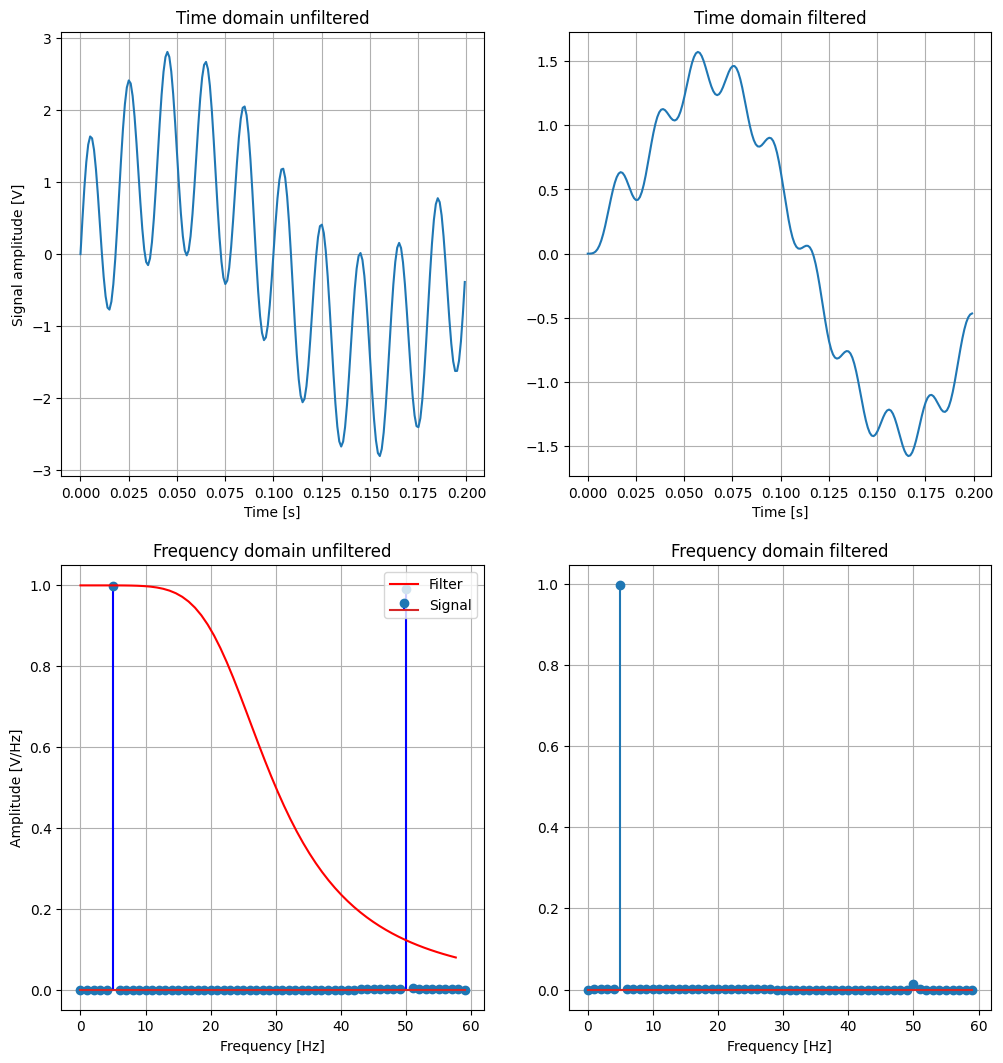
\includegraphics[width=1.0\columnwidth]{images/filter_example.png}
	\end{center}
	\caption{Filtering a signal. In the top-left figure there is a low-frequency signal polluted by a 50Hz signal. The frequency plot in the bottom-left shows these frequencies. By applying the low-pass filter as displayed in the bottom-left it is possible to filter out the higher 50Hz frequency. The resulting filtered signal can be seen in the top-right, showing that there is still a little bit of noise left. This is also visible in the bottom right showing the frequency contents of the signal after filtering}
	\label{fig:filter_example}
\end{figure}

A digital filter consists of a set of values called the filter coefficients. The input (measurements) is multiplied with the filter coefficients to create the output. That is, the latest measurement is multiplied with the first filter coefficient, the previous measurement is multiplied with the second filter coefficient, and so on. This can also be interpreted as multiplying each filter coefficients with a delayed input sample. Figure~\ref{fig:wiki_digital_filter_working} shows the working and standard notation of a digital filter.
By carefully choosing the number and value of filter coefficients it is possible to attenuate specific frequencies while not influencing other frequencies such as the effect shown in \ref{fig:filter_example}. Analog signals and filters are conventionally presented as a continuous function of time (e.g. $x(t)$). Digital signals and filters are discrete rather than continuous, and are conventionally presented as a function of samples (e.g. $x(n)$). The variable $n$ describes the n'th sample of the signal. Converting a continuous signal to a discrete signal is done through the process of sampling the continuous signal at equidistant points in time: $s(n)=s(n*\Delta t)$ \cite{linear_systems_and_signals}.

\begin{figure}[h!t]
	\begin{center}
		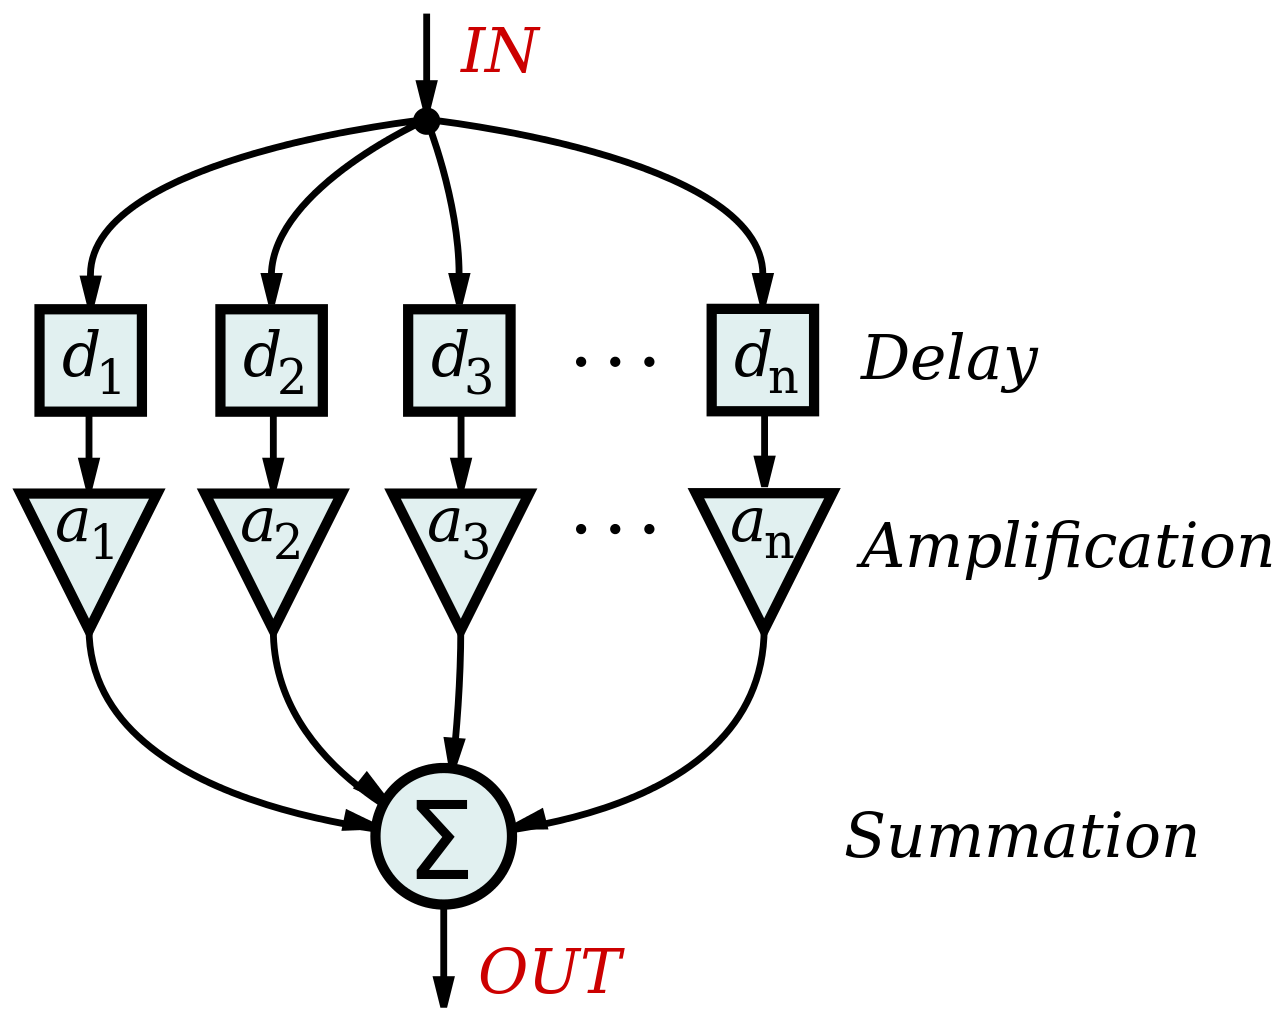
\includegraphics[width=0.4\columnwidth]{images/wikipedia_fir_digital_filter.png}
	\end{center}
	\caption{The functioning of a digital filter. The filter coefficient at index $i$ is multiplied by the input that is delayed $i$ samples \cite{wikipedia:digital_fir_filter_image}}
	\label{fig:wiki_digital_filter_working}
\end{figure}

\subsection{Static filters, Wiener filter, Adaptive filters}\label{sec:filters_theory}
The main difference between the different presented filter types is the way of calculating the filter coefficients. If a filter is static (e.g. high-pass, low-pass, band-pass, or band-stop) it simply means that the number of filter coefficients and the values of the filter coefficients are predetermined. These filters are very popular due to their simplicity in terms of finding the value of the filter coefficients. 

A Wiener filter aims to produce an estimate of a target process by linear time-invariant filtering of a noisy signal using knowledge of the spectrum of the stationary noise and target process assuming additive noise \cite{wiki:Wiener_filter,lecture_adaptive_filters_1}. Figure~\ref{fig:wiener_filter_diagram} shows the use of a Wiener filter. It is assumed that the noise component $v(n)$ is correlated to the noise component in the input signal in input $d(n)$ and uncorrelated to the desired signal $s(n)$. The Wiener filter coefficients aim to minimize the correlated signals, leaving only the desired signal as the 'error'. It is the optimal solution in terms of mean square error to statically filtering additive noise from a signal. The filter is constructed from the cross-correlation between an input sample and a noise sample, and the auto-correlation of the noise sample.

\begin{figure}[h!t]
	\begin{center}
		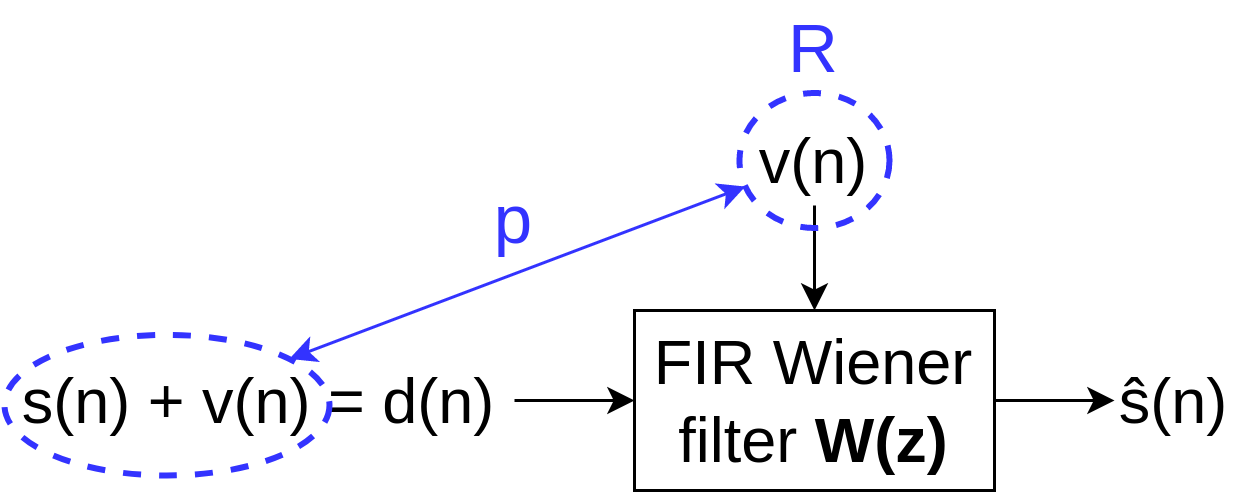
\includegraphics[width=0.7\columnwidth]{images/wiener_filter_diagram.png}
	\end{center}
	\caption{Diagram that illustrates the functioning of a Wiener filter. $s(n)$ is the desired signal, $v(n)$ is the additive noise, and $d(n)$ is the combination of desired signal and noise \cite{wiener_filter_system_identification}}
	\label{fig:wiener_filter_diagram}
\end{figure}

$s(n)$ is the target signal, $v(n)$ is the additive noise. The goal of the Wiener filter is to find an estimate $\hat{s}(n)$ of the target signal $s(n)$ using spectral knowledge of $v(n)$ and of the additive combination of $s(n)+v(n)$. The target signal estimate $\hat{s}(n)$ is also called the 'error' as it is the part that is left over after applying the Wiener filter. $w$ presents the wiener filter coefficients.
  \begin{equation}\label{eq:start_wiener}
    \hat{s}(n) = (s(n) + v(n)) - \hat{v}(n) = d(n) - \boldsymbol{w}^T v(n)
  \end{equation}
Calculate the square of the error \cite{lecture_adaptive_filters_1}
\begin{equation}
    \hat{s}^2(n) = (d(n) - \boldsymbol{w}^T v(n))^2
\end{equation}
\begin{equation}
    \hat{s}^2(n) = d^2(n) - 2d(n)\boldsymbol{w}^T v(n) + \boldsymbol{w}^T v(n)\boldsymbol{w}^T v(n)
\end{equation}
\begin{equation}
    \hat{s}^2(n) = d^2(n) - 2 \boldsymbol{w}^T d(n) v(n) + \boldsymbol{w}^T v(n) v^T(n) \boldsymbol{w}
\end{equation}
Take the mean of both sides to end up with the Mean Square Error (MSE) \cite{lecture_adaptive_filters_1}
\begin{equation}
    E\left(\hat{s}^2(n)\right) = E\left(d^2(n)\right) - 2 \boldsymbol{w}^T E\left(d(n) v(n)\right) + \boldsymbol{w}^T E\left(v(n) v^T(n)\right) \boldsymbol{w}
\end{equation}
Redefine terms of the equation \cite{lecture_adaptive_filters_1}
\begin{align}
&J(\boldsymbol{w}) \                  &=& E(\hat{s}^2(n))  &=& \text{MSE (scalar)} \label{eq:wiener_mse_def}\\
&\sigma^2 \           &=& E(d^2(n))        &=& \text{Power of }d(n) \text{ (scalar)} \\
&\boldsymbol{p} \      &=& E(d(n) v(n))     &=& \text{M-by-1 Cross-correlation vector between } d(n) \text{ and } v(n)  \\
&\boldsymbol{R} \      &=& E(v(n) v^T(n))  &=& \text{M-by-M Auto-correlation matrix of } v(n)
\end{align}
Insert redefined terms into the equation to form the total equation for Mean Square Error \cite{lecture_adaptive_filters_1}
\begin{equation}
    J(\boldsymbol{w}) = \sigma^2 - 2 \boldsymbol{w}^T \boldsymbol{p} + \boldsymbol{w}^T \boldsymbol{R} \boldsymbol{w}
\end{equation}
To find the filter coefficients that result in minimum MSE we take the derivative of the MSE with respect to each filter coefficient. The derivation of this process is quite lengthy but can be found in \cite{proakis_manolakis_1996}. The resulting final solution is called the Wiener-Hopf equation \cite{lecture_adaptive_filters_1} and is also shown in Equation~\ref{eq:wiener_hopf}
\begin{equation}\label{eq:end_wiener}
    \frac{\delta J}{\delta w_i} = 0, i = 0, 1, ... M-1 \ \rightarrow \ \boldsymbol{R} \boldsymbol{w_{opt}} = \boldsymbol{p} \ \rightarrow \ \boldsymbol{w_{opt}} = \boldsymbol{R}^{-1}\boldsymbol{p} \text{\cite{lecture_adaptive_filters_1}}
\end{equation}


The mathematical derivation for finding the optimal filter coefficients is given in equations \ref{eq:start_wiener} to \ref{eq:end_wiener}. The conclusion is that the optimal filter coefficients are calculated by multiplying (dot-product) the inverse of the auto-correlation of signal+noise and the cross-correlation between signal+noise and noise. In sEMG, the signal+noise is measured at the point of muscle contraction while the noise can be measured separately from a different body part that does not experience contraction. This separately measured noise has similar frequency characteristics as the noise included in the signal+noise as it experiences the same amplifier noise and environment noise. The resulting frequency domain definition of the optimal Wiener filter is defined in Equation~\ref{eq:wiener_filter_frequency_behaviour}\cite{stanford_wiener_filter}.

\begin{equation}
    H_{opt}(z) = \frac{\Phi_{s}(z)}{\Phi_{s}(z) + \Phi_{v}(z)}
    \label{eq:wiener_filter_frequency_behaviour}
\end{equation}

Assuming that the calculated Wiener filter approximates the optimal Wiener filter, multiplying the filter (in frequency domain) with the signal+noise input will result in an approximation of the signal as seen below.

\begin{align}
    \hat{\Phi_{s}}(z) & \ = \ \hat{H_{opt}}(z) \ \cdot \ (\Phi_{s}(z) + \Phi_{v}(z)) \label{eq:wiener_filter_frequency_application_1} \\
    & \ = \ \frac{\hat{\Phi_{s}}(z)}{\hat{\Phi_{s}}(z) + \hat{\Phi_{v}}(z)} \ \cdot \ (\Phi_{s}(z) + \Phi_{v}(z)) \label{eq:wiener_filter_frequency_application_2}\\
    & \ \approx \ \Phi_{s}(z) \label{eq:wiener_filter_frequency_application_3}
\end{align}

The Wiener filter requires both the signal and the noise to be stationary, i.e. the spectral density does not change over time, and results in a linear time-invariant filter \cite{stationary_processes_definition} \cite{difference_stationary_nonstationary}. If the signal and noise were not stationary then the approximated frequency spectrum of signal+noise is not the same as the actual frequency spectrum of signal+noise which means they no longer cancel out in Equation~\ref{eq:wiener_filter_frequency_application_2} and Equation~\ref{eq:wiener_filter_frequency_application_3} no longer holds.
As an example a Wiener filter was made from the signal as seen in Figure~\ref{fig:sEMG_signal_example}. The time span from 0-2 seconds is taken as the 'noise', and the time span from 5-7 seconds is taken to be signal+noise. From these a Wiener filter is constructed and can be seen in Figure~\ref{fig:wiener_filter_response}.

\begin{figure}[h!t]
	\begin{center}
		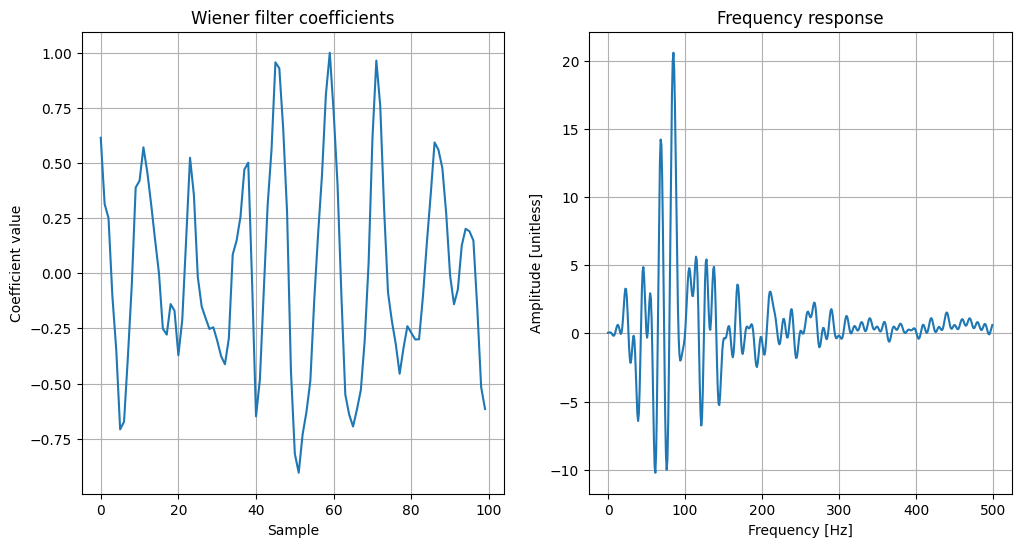
\includegraphics[width=1.0\columnwidth]{images/wiener_filter_response.png}
	\end{center}
	\caption{Sample values and frequency responses of a Wiener filter}
	\label{fig:wiener_filter_response}
\end{figure}

\begin{figure}[h!t]
	\begin{center}
		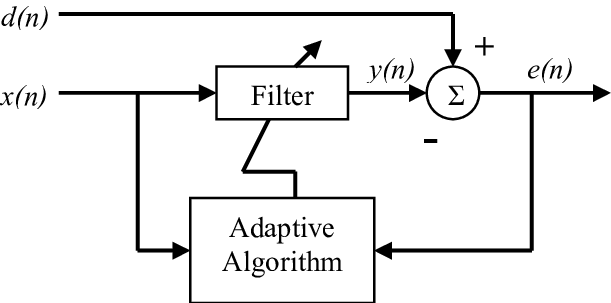
\includegraphics[width=1.0\columnwidth]{images/adaptive_filter_block_diagram.png}
	\end{center}
	\caption{Block diagram of an adaptive filter \cite{introduction_optimal_signal_processing}}
	\label{fig:adaptive_filter_diagram}
\end{figure}

Adaptive filters is a class of filters where the filter coefficients are adjusted over time to attempt to find an optimal solution even without knowing the spectral properties of the signal beforehand \cite{adaptive_filter_and_applications}. Adaptive filters adjust the filter coefficients by decreasing the error that remains after applying the filter. A diagram describing this process can be found in Figure~\ref{fig:adaptive_filter_diagram}. 
One type of adaptive filter is the Least Mean Square (LMS) algorithm. Where a Wiener filter finds an optimal solution by using cross-correlation and auto-correlation, the adaptive LMS algorithm converges to the optimal solution (i.e. the solution found by the Wiener filter given complete knowledge of the spectral domain) using gradient descent. Filter coefficients will never reach $w_{opt}$ but instead oscillate around it. The mathematical definition for calculating the filter coefficients is given, derived from the work of J. Orfanidis \cite[Ch. 7.3]{introduction_optimal_signal_processing} and lectures by S. Safapourhajari \cite{lecture_adaptive_filters_2}. Again it is assumed that there is an input signal ($d(n)$) consisting of a desired signal ($e(n)$) and additive noise ($x(n)$), as well as a separate measure of the noise that is correlated with the noise in the input signal but uncorrelated with the desired signal.

Taking the definition of the MSE (which is the cost function we're trying to minimize) as defined in Equation~\ref{eq:wiener_mse_def}
\begin{equation}
    J(w) = E(e^2(n)) = E[(d(n) - wx(n))^2)]
\end{equation}
To calculate the expected value of the square of the error we would normally need statistics over a large block of data. An approximation of the expected value can be made by using a smaller set of data. This can be done by taking the current samples as the estimates of the mean
\begin{equation}
    E(e^2(n) ~ e^(n)
\end{equation}
\begin{equation}
    E((d(n) - wx(n))^2)) ~ (d(n) - wx(n))^2
\end{equation}

To find $w$ that minimizes the MSE we can take the derivative of MSE with respect to $w$ for every sample $n$
\begin{equation}
    \frac{\delta J}{\delta w} = 2(d(n) - wx(n)) \frac{\delta(d(n) - wx(n))}{\deta w} = -2e(n)x(n)
\end{equation}
This results in the following weight-adjusting algorithm
\begin{equation}
   w(n+1) = w(n) + 2 \mu e(n)x(n)
\end{equation}
\begin{equation}
    \textrm{w(n+1)}=\left.w(n)-\mu \frac{\delta J}{\delta w}\right\rvert_{\textrm{w(n)}}
\end{equation}


This algorithm is implemented by performing the following steps. \\
The estimated value for signal+noise is computed from the filter and noise
\begin{equation}\label{eq:adaptive1}
    \hat{x}_n = w(n)\cdot y(n)
\end{equation}
The error is calculated by taking the difference between the expected signal+noise value and the measured signal+noise value.
\begin{equation}\label{eq:adaptive2}
    e(n) = x(n) - \hat{x}_n
\end{equation}
The coefficients are calculated for the next iteration
\begin{equation}\label{eq:adaptive3}
    w(n+1) = w(n) + 2 \mu e(n) x(n)
\end{equation}

The steps in equations \ref{eq:adaptive1}-\ref{eq:adaptive3} are repeated for every sample.

In the presented equations a constant $\mu$ was present, this is called the convergence coefficient. Determining the value of the convergence coefficient $\mu$ is a double-edged sword. On the one hand it determines how fast gradient descent is traversed, and thus how fast the filter coefficients converge to the optimal filter coefficients. Ideally this happens as fast as possible, and thus the convergence coefficient must be as large as possible. On the other hand it was previously mentioned that the filter coefficients will never reach the optimal filter coefficients but instead oscillate around this value. The convergence coefficient also determines how large this oscillatory behaviour is, and thus to achieve an accurate estimation of the optimal filter the convergence factor should be as small as possible. 

A problem presented by the basic LMS algorithm is that scaling the input also results in scaling the error term calculated in Equation~\ref{eq:adaptive2}. This makes it difficult (if not impossible) to find a convergence factor that functions across a wide range of possible scaled inputs. A solution to this problem is found in the work of Haykin \cite{adaptive_filter_theory} in the form of the Normalized LMS filter. This normalizes the power of the input signal before multiplying the input with the error and convergence factor. This is done by dividing the input signal with the the dot product of the input signal with itself. It turns Equation~\ref{eq:adaptive3} into Equation~\ref{eq:adaptive4} \cite{adaptive_filter_theory}.

\begin{equation}\label{eq:adaptive4}
    w(n+1) = w(n) + 2 \mu e(n)  \frac{x(n)}{x(n) \cdot x(n)}
\end{equation}

Common applications of adaptive filters include speech recognition, echo cancellation, and headphones employing active noise cancellation \cite{active_noise_cancellation_wiener_filter,wiener_vs_adaptive_realtime_noisecancellation}.

\subsection{FIR vs IIR}
Another subdivision within filter design is concerned with the type of possible responses to a specific input (impulse) and whether or not this can go to infinity.

The previously discussed filters were all described as Finite Impulse Response (FIR) filters. This means that the output is the result of multiplying the filter coefficients with the input. This type of filter is always stable and the output can never go to infinity as long as the input does not go to infinity.

An Infinite Impulse Response filter calculates the output using two sets of filter coefficients. The first set of filter coefficients is used to multiply with the input just like a FIR filter, but the second set of filter coefficients is used to multiply with previous \textit{outputs}. This means that there is now a feedback loop in the system, and a system with feedback can become unstable. Unstable in this case means that there is a possibility of positive feedback loop where increasing output values result in future output values also increasing, eventually going to infinity. Even though this feedback and possible instability may sound like a downside, it also results in shorter filter length and thus fewer computations required per filter operation. This could especially provide beneficial in low memory and low compute power environments like in prostheses \cite{fir_vs_iir}.

Both static and adaptive filters can be implemented as both FIR or IIR filters. An adaptive IIR filter offers the potential to meet desired performance levels with much less computational complexity. However, the possibility for the system to become unstable combined with the fact that filter coefficients are adjusted automatically leads to a high-risk high-reward scenario due to a loss of control and hard to predict behaviour \cite{digital_signal_processing_handbook}.

\begin{figure}[h!t]
	\begin{center}
		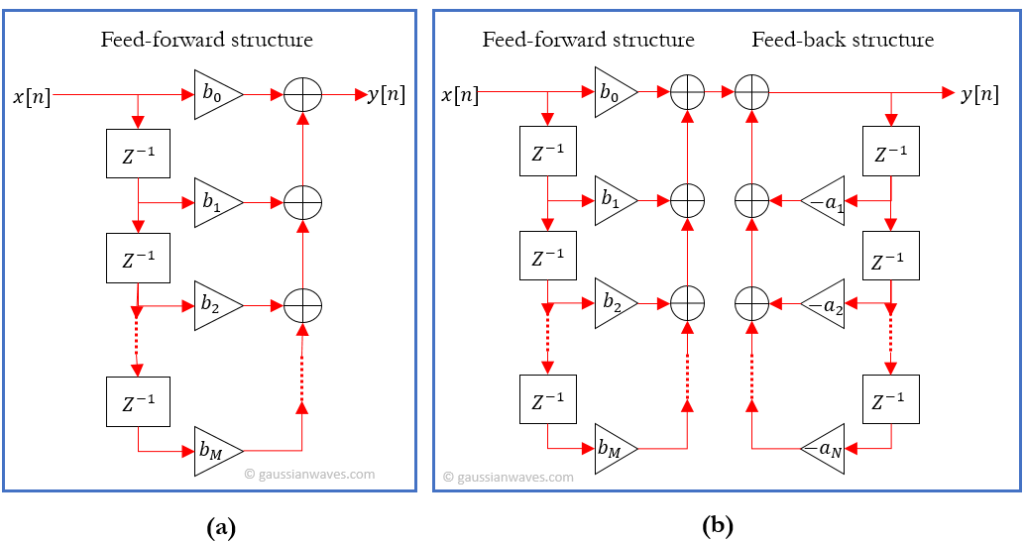
\includegraphics[width=1.0\columnwidth]{images/fir_vs_iir_diagram.png}
	\end{center}
	\caption{A diagram displaying the difference between Finite impulse response filters, only using previous input, and Infinite impulse response filters, using previous inputs and previous outputs resulting in a feedback loop \cite{fir_vs_iir_diagram}}
	\label{fig:fir_vs_iir_diagram}
\end{figure}


\section{Pre-whitening}
During literature research it was noticed that it was not uncommon for literature to mention something along the lines of "including a temporal whitening filter [...] improves the performance of the amplitude estimate" \cite{single_site_emg_amplitude_estimation,adaptive_whitening,emg_whitening}. However, an intuitive explanation of \textit{why} whitening works was consistently lacking. So to understand the reasoning behind whitening we need to take a short detour to the world of computer science and information theory.

Back in 1948 a mathematician, electrical engineer, and cryptographer named C.E. Shannon published a pioneering paper that formed the basis of information theory \cite{shannon}. In this paper it is shown that repetition does not carry information, and that the maximum information transfer occurs when a signal is truly random. Imagine a signal with only a single frequency component. After measuring a few samples of the signal the conclusion is drawn that this is a \SI{50}{\hertz} signal. Since it is possible to predict the value of every future measurement of the signal after drawing this conclusion it becomes unnecessary to continue measuring the signal because it will not give any new information. A repeating pattern is predictable, and predictable events carry no information.

The polar opposite of a signal containing a single frequency (and therefore predictable and carries little information) is a signal that contains all frequencies an equal amount. This is called a white noise signal and carries the maximum amount of information because there exists no repetition and therefore every sample carries new, unpredictable information.

Between the existence of a signal containing a single frequency, and a signal containing all frequencies (white noise), all other signals exist and have certain frequencies that are more 'present' than other frequencies. These signals have different degrees of predictability (and thus information density), and the degree of predictability is determined by how closely the frequency content resembles white noise.

Whitening is a filtering technique that tries to equalize the presence of frequency components in a signal to approximate white noise and thus increase information density. It reduces the random error and yields a larger dynamic range because the small frequency components that contribute to the 'randomness' of the signal but not so much to the value of the measurement sample become more present \cite[Ch. 5.4.9]{time_series_analysis_methods}\cite{single_site_emg_amplitude_estimation}. The serial correlation of the signal is decreased by reducing the presence of 'predictable' signals, which increases the randomness and thus information density \cite{serial_correlation_definition}. 

This previous information manifests itself in sEMG signal processing by the fact that the measured sEMG signal is not white. Some frequency components are much more present than others, but all frequencies equally contribute to the indication of muscle contraction. To get a more accurate indication of muscle contraction the signal should be whitened to increase the information of each sample.

Whitening in real-time is achieved through a digital filter with a frequency response that when multiplied with the sEMG signal frequency spectrum yields a white noise spectrum.

To summarize: Whitening reduces the power of repeating frequencies and increase the power of random frequencies in the signal. An example is given in Figure~\ref{fig:whitening_example}.

\begin{figure}[h!t]
	\begin{center}
		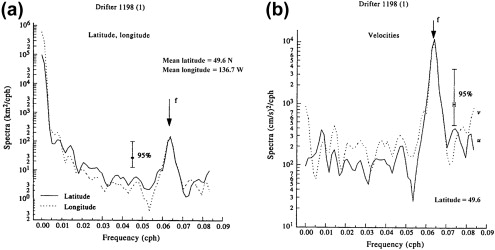
\includegraphics[width=1.0\columnwidth]{images/prewhitening_example.jpg}
	\end{center}
	\caption{An example of whitening a signal. The indicated peak contains the 'random' signal of interest. By whitening the powerful lower frequencies it is possible to give the information-carrying peak more presence on the signal \cite{time_series_analysis_methods}}
	\label{fig:whitening_example}
\end{figure}


\section{Envelope detection}

\begin{figure}[h!t]
	\begin{center}
		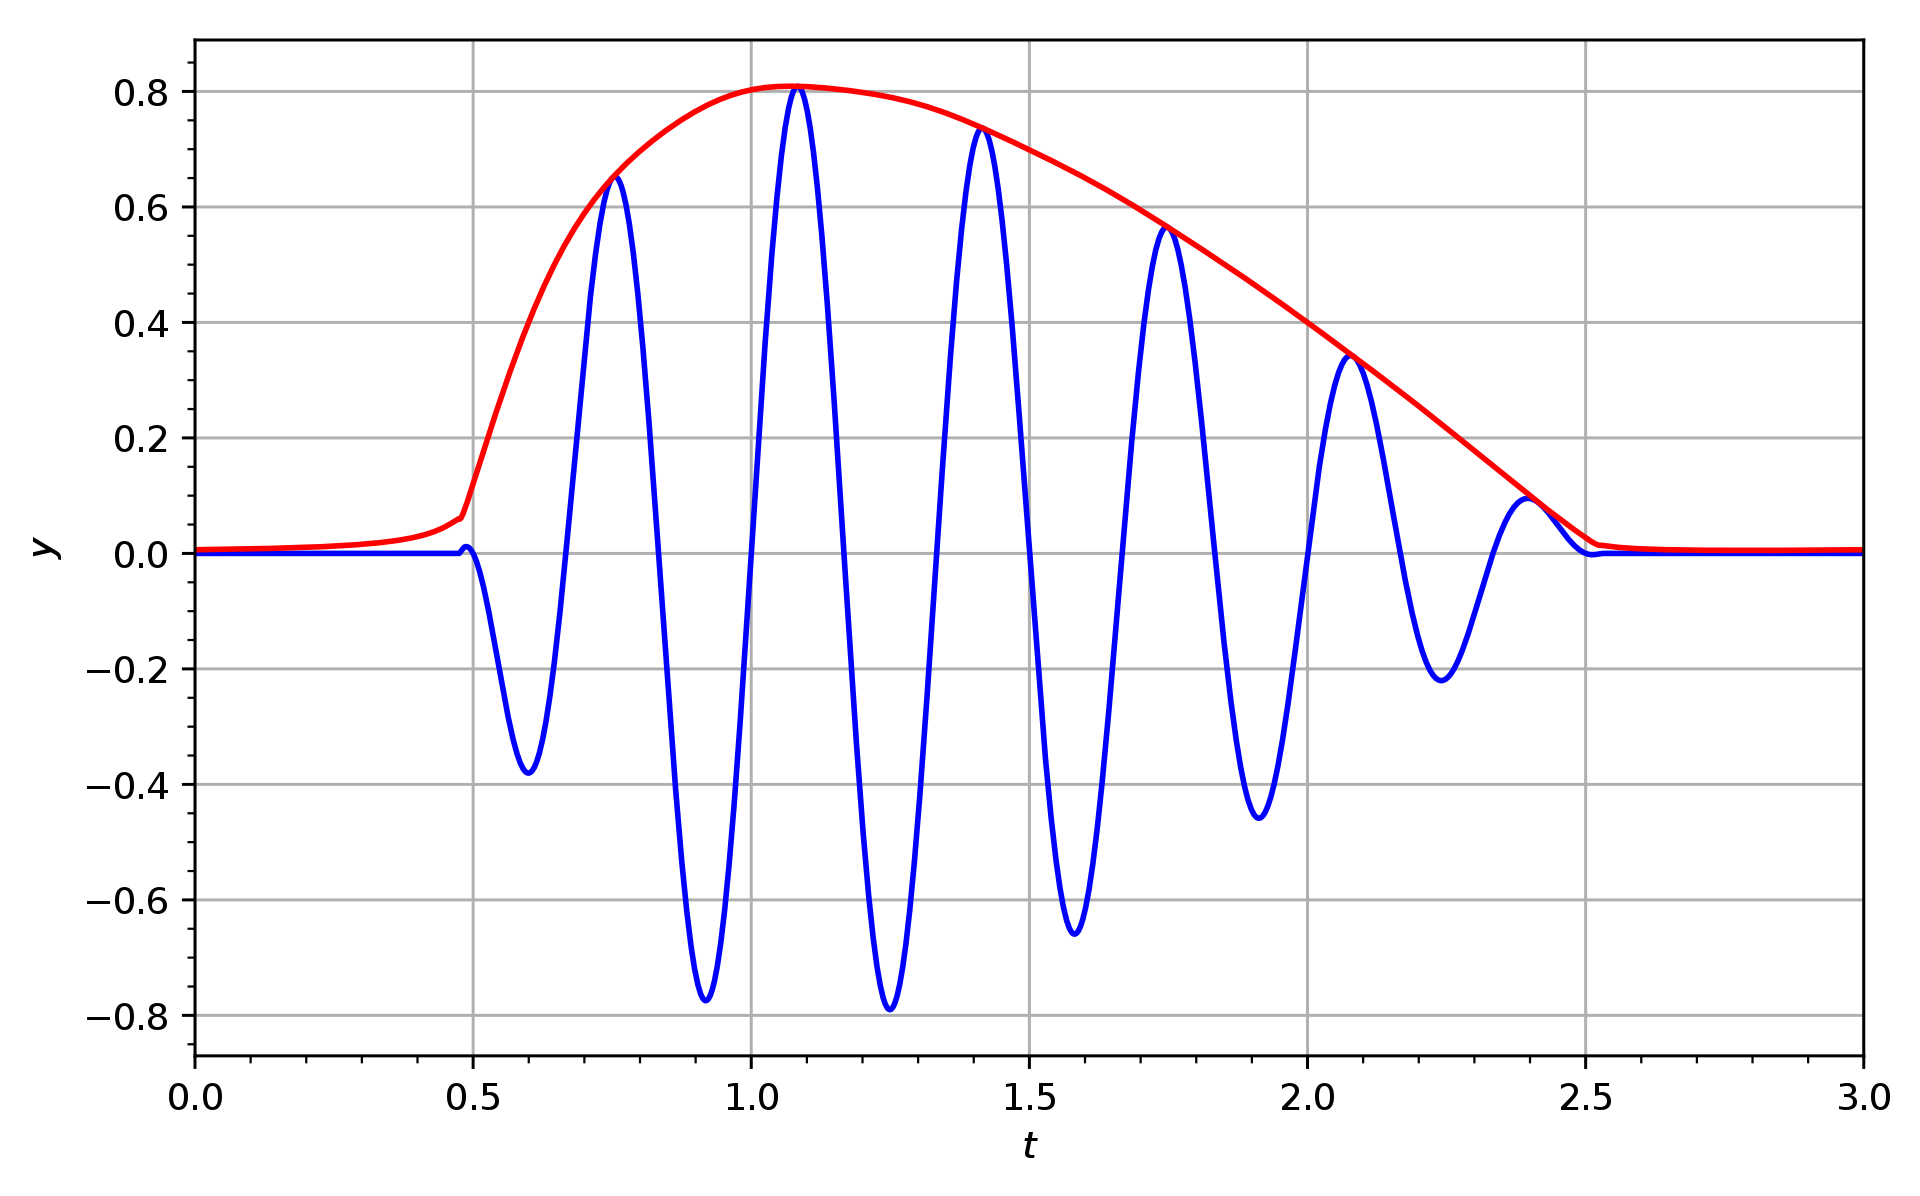
\includegraphics[width=0.7\columnwidth]{images/envelope_wikipedia.png}
	\end{center}
	\caption{Illustrating envelope detection of an analytical signal \cite{envelope_wikipedia}}
	\label{fig:envelope_wikipedia}
\end{figure}

\begin{figure}[h!t]
	\begin{center}
		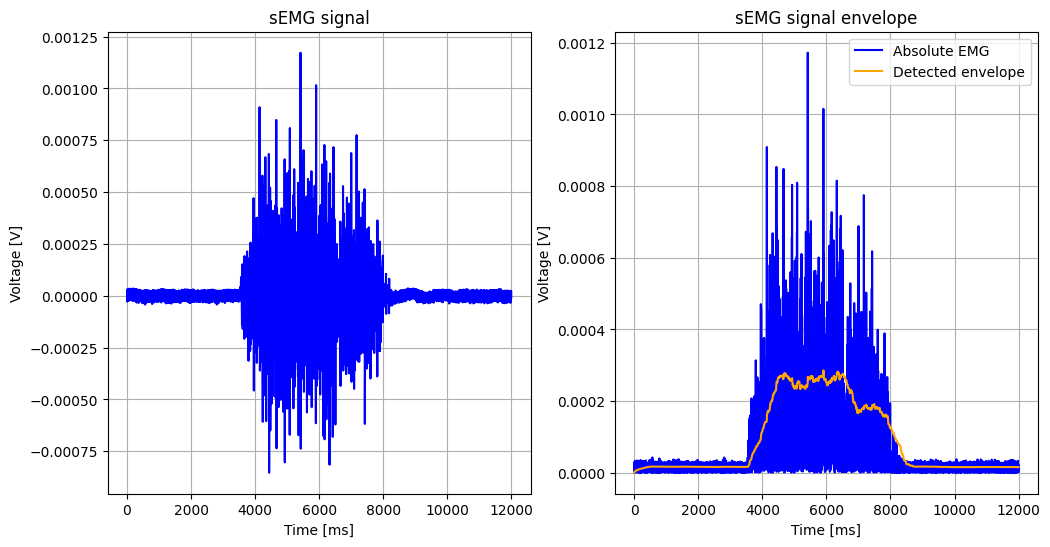
\includegraphics[width=1.0\columnwidth]{images/amplitude_force_estimation_example.png}
	\end{center}
	\caption{On the left a time-domain sEMG signal. On the right an example of envelope estimation is presented. By taking the absolute value of the sEMG signal on the left and calculating the envelope it is possible to make an estimation of muscle contraction. The next step would be force estimation but this requires two antagonistic muscles. This is discussed more in-depth in section \ref{section:force_estimation}}
	\label{fig:amplitude_estimation_example}
\end{figure}

The relation between the amplitude of a measured sEMG signal, the degree of contraction of a skeletal muscle and the exerted force is very complicated. However, the relationship between force and EMG amplitude during isometric contractions is usually linear or close to linear  \cite{interpreting_muscle_function_from_emg} \cite{adaptive_filter_dry_electrode}. This is the reason that in this report it is assumed that there exists a linear relation between force and sEMG signals.

Since the raw EMG signal consists of stochastic and unpredictable noise it is difficult to draw conclusions about the degree of muscle contraction when solely looking at individual samples \cite{semg_signals_analysis_and_applications}. By drawing an outline of the peaks of the signal a much more informative picture can be drawn. This is called an envelope and an illustration of this process can be found in Figure~\ref{fig:envelope_wikipedia}. In the case of more random sEMG signals it is preferred to perform full wave rectification on the signal before calculating the envelope so that all of the signal energy is taken into account \cite{semg_signals_analysis_and_applications}. Applying this concept to an sEMG signal can be found in Figure~\ref{fig:amplitude_estimation_example}.

Computationally envelope detection can be achieved in a number of different methods where "speed", or how much the detected envelope lags behind the true signal envelope, is traded against accuracy or noisiness \cite{dsp_good_bad_ugly}. A few different envelope detection techniques are discussed in \cite{rose2011electromyogram}.

\subsection{Moving average}
A moving average filter is a special type of FIR filter with coefficients that all have the value of $\frac{1}{n}$ where $n$ is the number of samples over which the average is taken. Thus the value of every smoothed sample is calculated to be the average of the previous $n$ samples. The upside of a moving average filter is that it introduces no phase distortion \cite{fir_filter_properties}, is very simple to implement, and require only addition to apply which is much faster than multiplication \cite{smith_moving_average_filters}. An illustration of the phase shift of a moving average filter is shown in Figure~\ref{fig:movingaverage_phaseshift}. An intuitive downside of a moving average filter is that its output lags behind the signal: a change in a static signal level is only properly reflected after $n$ samples. The sEMG signal must also be rectified before this method can be applied because EMG signal has approximately zero mean due to its oscillatory behaviour \cite{rose2011electromyogram}.

\begin{figure}[h!t]
	\begin{center}
		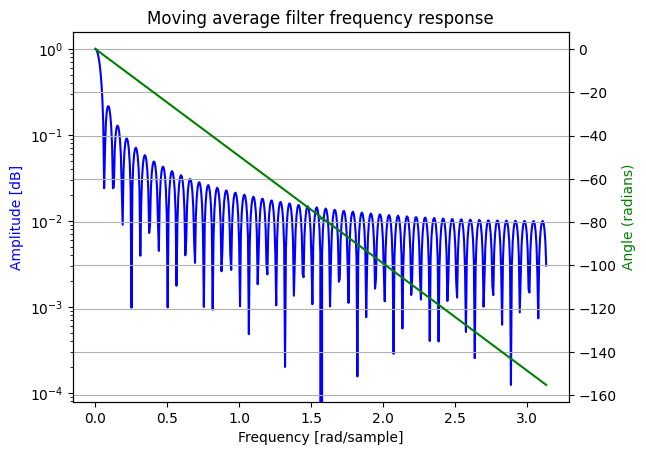
\includegraphics[width=0.7\columnwidth]{images/movingaverage_phaseshift.png}
	\end{center}
	\caption{Frequency response of a moving average filter. This particular filter consists of 100 coefficients all equal to 0.01. Notice how the filter has linear phase which indicates that there is no phase distortion due to the time delay of frequencies relative to another \cite{fir_filter_properties}}
	\label{fig:movingaverage_phaseshift}
\end{figure}



\subsection{IIR Low-pass filter}
A low-pass filter such as a Butterworth or Chebyshev can be used to determine the envelope of a rectified signal in a more 'responsive' (less lag) method compared to a moving average filter. The downside of this filter is that it introduces phase shift (as can be seen in Figure~\ref{fig:iirfilter_phaseshift}) unless applied in forward and backward direction \cite{rose2011electromyogram} which is not possible in real-time signals without introducing a static delay of a number of samples that equals the number of filter coefficients.

\begin{figure}[h!t]
	\begin{center}
		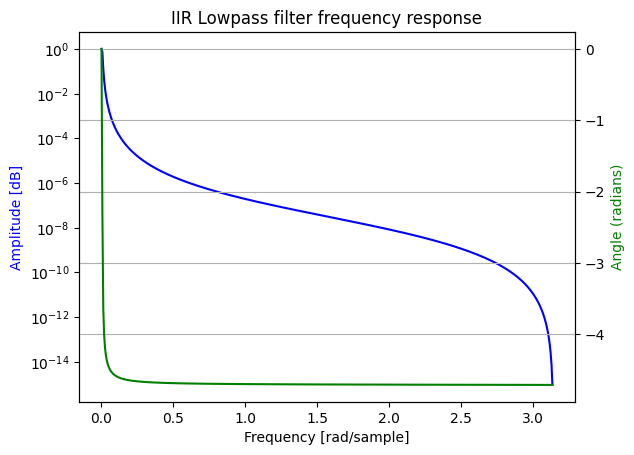
\includegraphics[width=0.7\columnwidth]{images/iirfilter_phaseshift.png}
	\end{center}
	\caption{Frequency response of an infinite impulse response (Butterworth) low-pass filter. The filter has a $f_{cut}$ of \SI{1}{Hz} and has a length of 3. Notice how the phase delay is \textit{not} linear and thus phase distortion is introduced}
	\label{fig:iirfilter_phaseshift}
\end{figure}

\subsection{Root Mean Square}
The Root Mean Square (RMS) of a signal is the square root of average power of a signal for a given period of time, a definition is given in Equation~\ref{eq:rms}. A useful property of RMS is that when it is applied to a signal with Gaussian distribution the RMS amplitude of the source is the same as the standard deviation of the distribution \cite{rms_standard_deviation}. In other words this means that RMS can extract the signal power of all frequencies in a signal in the time-domain if the frequencies are normally distributed. Since the probability density of surface EMG is approximately Gaussian, RMS should theoretically be the maximum likelihood estimator of EMG amplitude \cite{semg_signals_analysis_and_applications}.

\begin{equation}
    RMS = \sqrt{\frac{1}{n} (x[1]^2 + x[2]^2 + \cdots + x[n]^2)}
    \label{eq:rms}
\end{equation}

\section{Standard sEMG signal processing}\label{section:standard_semg_processing}
A conventional static real-time sEMG signal processing chain is described in \cite{muscle_force_estimation}. The relevant steps are as follows:
\begin{itemize}
    \item Remove DC component from signal
    \item Band-pass filter 20-\SI{300}{\hertz}
    \item Notch filter at \SI{50}{\hertz}
    \item Half-wave rectification
    \item Low-pass filter for envelope detection
\end{itemize}

This signal processing chain will also be tested in this report and compared to alternative techniques.